\subsection{Vernetzte SBCs}

Abbildung \ref{fig:arch_03} zeigt die Komponenten der vernetzten SBC-Geräte. Eine Verarbeitungsanwendung kann eine beliebige Anzahl von Prozessoren erhalten, die jeweils ihre Dienste über den Zeroconf/Bonjour-Daemon im Netzwerk anbieten. Das Zeroconf/Bonjou-Daemon wird als teil des Betriebsystems hier dargestellt. Die Zeroconf/Bonjour-Daemon sendet die Verfügbarkeit, der Verarbeitung-Art und die Portnummern von jedem der verfügbaren Prozessoren.

\begin{figure}[H]
    \centering
    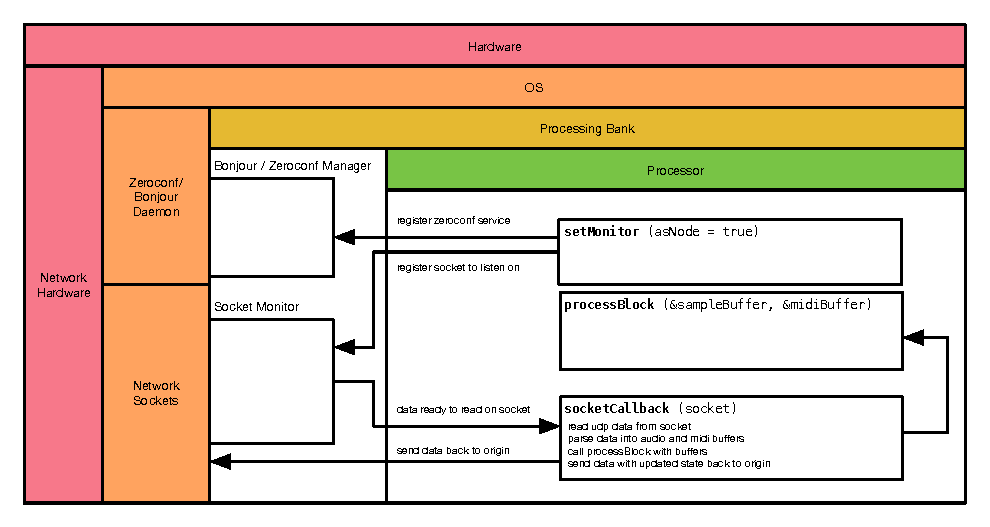
\includegraphics[width=\textwidth]{assets/architecture_03.pdf}
    \caption{SBC Processor Überblick}
    \label{fig:arch_03}
\end{figure}

Der Prozessor übergibt eine offene Socket an einen Socket-Monitor und registriert sich als dazugehörende Socket-Zuhörer-Objekt. Die Socket-Monitor besitzt eine Reihe von Sockets und einen Verweis auf jeden Zuhörer. Es führt eine "select" Funktion auf der Reihe von Socket und wartet. Wenn Daten an einem der Sockets eintreffen, erwacht der "select" Funktion und der Socket Monitor benachrichtigt den entsprechenden Socket-Zuhörer-Objekte über eine Rückruffunktion, das Daten zu verfügung stehen.

Der entsprechende Prozessor wird über die Rückruffunktion benachrichtigt, liest die Daten, entpackt die Audio-, Zustands- und MIDI-Daten, und führt den processBlock Funktion aus. Die Ergebnisse und aktualisierte Zustandsinformation werden am Sender zurück geschickt.

